\documentclass[12pt]{article}

\usepackage{sbc-template}

\usepackage{graphicx,url}

%\usepackage[brazil]{babel}   
\usepackage[latin1]{inputenc}  

     
\sloppy

\title{PlantGoshi\\ Projeto Integrador III - Sistema Aut\^onomo}

\author{Anderson J. Silva, Felipe R. de Luca, Nelson J. Dressler }


\address{Bacharelado em Ci\^encia da Computa\c c\~ao -- Centro Universit\'ario Senac - Santo Amaro \\
  S\~ao Paulo - SP - Brasil \\ 2015
}
\begin{document} 

\maketitle
     
\begin{resumo} 
[ ... ]
\end{resumo}

\section{Introdu\c c\~ao}

 O Projeto consiste num jogo de simula\c c\~ao de cria\c c\~ao
 de plantas e do seu cuidado contra a presen\c ca de invasores e/ou criaturas nocivas \`a sua
 sobreviv\^encia no seu habitat natural, a terra.
 O jogador ter\'a poderes por interm\'edio de uma varinha m\'agica e, ao longo do jogo, dever\'a utiliz\'a- los para alimentar e
 aprimorar a planta ou a \'arvore e tamb\'em combater as pragas aparentes atrav\'es
 de intera\c c\~ao com diferentes cores emitidas pelo LED.
 

 Os frutos nascem verdes em pontos rand\^omicos e demoram um tempo x para seguir para a segunda etapa.
 Se o fruto no estado verde n\~o for "regado" (ou, poder de música) depois de um tempo determinado,
 ele vai ficar maduro com praga ou ficar\'a estragado. Isso for\c ca o usu\'ario a usar o poder de "regar"
 (ou, poder de m\'usica) no fruto.
 
 Quando o fruto fica maduro, depois de um tempo x ele cria praga, for\c cando o usu\'ario a usar o poder
 de "remover" para eliminar a praga do fruto maduro. 
 
 Com o fruto maduro e sem praga o usu\'ario poder\'a usar o poder de  "colher" para  colher o fruto e somar pontos. 
 Se o usu\'ario colher fruto verde, maduro com praga ou estragado ele perde pontos.
 Caso deixe o fruto estragar tamb\'em pontos s\~ao descontados. Depois que uma quantidade x de frutos estragar
 o jogo termina.
 
\section{Estrutura principal do jogo}
\subsection{Layout}
Na parte inferior, aparecem os \'icones com os poderes dispon\'iveis, cada uma com uma cor diferente
(azul: hidratar, vermelho: combater, verde: tocar a m\'usica); na parte superior esquerda,
uma barra de progresso do crescimento da \'arvore (branco, verde claro, verde escuro);
na parte superior central, uma barra de progresso da qualidade dos frutos; superior direita,
uma barra de progresso da sa\'ude da planta; esquerdo central, um painel de controle entre o calor,
a hidrata\c c\~ao da \'arvore e ocorr\^encia de pragas.

\subsection{Componentes de Tela}
\begin{itemize}
\item Barras de progresso de crescimento da \'arvore, amadurecimento dos frutos e de sa\'ude da planta;
\item Painel de Controle com 3 dire\c c\~oes (\'agua, calor e praga);
\item \'Icones de poderes; \'Arvore (tronco central, galhos, ra\'izes, folhas, frutos), Pragas (ervas daninhas e larvas) e Cesta;
\item Ferramentas de intera\c c\~ao (m\~aozinha, nota musical e gota d'agua).
\end{itemize}

\subsection{Jogabilidade}
o jogador acessa os poderes com a sua varinha conectada ao Arduino encostando
o objeto na tela e poder\'a aplicar o poder selecionado em qualquer parte da tela,
encostando novamente. Para isso, estar\~ao presentes duas c\^ameras: uma frontal
apontado para o jogador (altura e largura) e outra lateral (profundidade).
Para representar os poderes selecionados no momento, a varinha ter\'a um LED
correspondente a cor do poder (branco: nada selecionado, azul, vermelho e verde).

\subsection{Etapas}
\begin{enumerate}
\item \textbf{Nascimento e Crescimento da \'Arvore:} \'e contemplado pelo processo desde o plantio
 da semente at\'e a \'arvore crescer e brotar atingindo um tamanho razo\'avel e que j\'a det\'em a
 capacidade de criar galhos e plantas;
\item \textbf{Amadurecimento dos Frutos:} \'e composto pelo momento onde a planta j\'a
 come\c ca a dar seus primeiros frutos;
\item \textbf{Colhimento dos Frutos:} \'e o momento no qual os frutos cresceram e amadureceram
 o suficiente para serem recolhidos e depositados numa cesta.
\end{enumerate}

\subsection{Simula\c c\~ao}
Iniciando o jogo, a \'arvore est\'a com suas ra\'izes dentro do solo e um pequeno e fino caule
 brotando. Nesse momento, 2 poderes aparecem na tela: azul (lado esquerdo) e vermelho (centro)
 (O poder da nota musical fica desabilitado). Passa um pequeno per\'iodo de tempo e o painel
 de controle come\c ca a tender para a cor azul, indicando a necessidade de regar planta.
 O jogador seleciona com a varinha a gota d'agua (encostando na tela), o LED da varinha
 troca de cor (de branco para azul) e come\c ca a aplicar a \'agua na planta para que cres\c ca
 verticalmente (encostando na tela). A c\^amera lateral detecta a sele\c c\~ao da varinha e
 a aplica\c c\~ao. A c\^amera frontal detecta a posi\c c\~ao (coordenada x, y) que a varinha
 tocou \`a tela. Ap\'os alguns segundos (10 segundos) o poder de \'agua termina e os \'icones
 ficam travados por um tempo (dependendo do n\'ivel) para recarregar e novamente estar
 habilitado na tela. A barra de progresso do crescimento da \'arvore avança um pouco
 (ainda permanecendo na cor branca) e a barra de controle centraliza novamente, indicando
 equil\'ibrio das for\c cas. Ao mesmo tempo, a barra de sa\'ude tamb\'em avan\c ca um pouco.

 Ao mesmo tempo, aparecem ervas daninhas crescendo junto a planta. O painel de controle indica
 a necessidade de aplicar fogo nas mesmas, tendendo para a cor amarela. Nesse momento, o jogador
 seleciona a m\~aozinha e aplica o fogo para queimar as ervas. Ap\'os alguns segundos (10 segundos),
 o poder termina e novamente todos ficam travados por um tempo (dependendo do n\'ivel) desabilitado.
 Ao final, o painel de controle \'e centralizado novamente.
 
 Deve se ter o cuidado para n\~ao usar excessivamente o poder do fogo para n\~ao queimar a planta tamb\'em.
 Isso ser\'a indicado no painel de controle com o indicador tendendo para a cor vermelha.
 
 Assim que a \'arvore estiver crescido consideravelmente (a definir), os poderes ficam dispostos na parte
 inferior da tela da seguinte maneira: azul (lado esquerdo), verde (direito) e vermelho (centro).

 Al\'em disso, a medida que o jogo segue come\c cam a aparecer algumas notas musicais flutuando na tela.
 O jogador seleciona a nota musical e aplica na planta para melhorar o crescimento e florescimento da \'arvore
 (espessura) e o crescimento qualitativo dos frutos. Novamente, o poder dura quest\~ao de segundos
 (10 segundos) at\'e que termina e, logo em seguida, todos ficam travados por algum tempo (dependendo do n\'ivel).

 Ao mesmo tempo, o jogador deve regar a \'arvore (azul) para que continue crescendo (verticalmente) e combater
 as pragas que come\c cam a aparecer nas folhas e flores (vermelho).
 
 Nesse momento, come\c cam a crescer os primeiros frutos e, para isso, \'e necess\'ario continuar regando
 a planta, combatendo as pragas e tocando as notas musicais (crescimento dos frutos).

 Finalmente, o jogador atinge a \'ultima parte do jogo que \'e constitu\'ida pela colheita dos frutos,
 j\'a em sua condi\c c~ao ideal para tal a\c c\~ao.

 Nessa \'ultima etapa o jogador deve ser r\'apido para colher os frutos sem que apodre\c cam (azul, lado direito)
 e, ao mesmo tempo, combater as pragas que crescem e progridem a cada instante (vermelho, lado esquerdo).
 Essas dever\~ao ser realizadas atendendo ao tempo limite imposto sobre aquela etapa (f\'acil: 2 min; m\'edio:
 1 min; difícil: 30 segs).
 
 Novos frutos v\~ao nascendo ao mesmo tempo que outros v\~ao amadurecendo at\'e apodrecer. Ent\~ao, \'e
 necess\'aria a percep\c c\~ao de tudo o que ocorre naquele instante, para saber qual for\c ca selecionar
 e qual jogada escolher, visando a sa\'ude da \'arvore e a qualidade dos frutos.
 
 Ao fim dessa etapa, \'e atribu\'ida uma pontua\c c\~ao ao jogador pela atua\c c\~ao completa e o jogo se
 d\'a por encerrado.

\section{Algoritmos}
\subsection{Vis\~ao Computacional}

Compreendendo a parte de vis\~ao computacional, est\'a sendo feito um levantamento bibliogr\'afico
referente ao processamento digital de imagens, reconhecimento de padr\~oes em imagens, opera\c c\~oes
aritm\'eticas e um estudo aprofundado sobre o modelo HSV (Hue, Saturation e Value ou Brightness).

\subsection{Espa\c co de cores}
\subsubsection{Espa\c co de cor HSV}
Foi poss\'ivel executar alguns testes sobre os pixels capturados da imagem de uma c\^amera,
descobrindo o grau da cor pura (Matiz) e as faixas representada por cada cor, a porcentagem de satura\c c\~ao
da cor (Pureza) e a porcentagem de brilho (Valor), apenas convertendo do modelo RGB para o HSV.

Foram realizadas tamb\'em algumas opera\c c\~oes sobre os pixels como a redu\c c\~ao da quantidade
das poss\'iveis cores aparentes pela imagem, dividindo a composi\c c\~ao do RGB por um fator (constante).
Foi poss\'ivel perceber que quanto maior o fator, menor a quantidade de cores poss\'iveis.

\subsubsection{Escala de cinza}
Utilizamos convers\~ao do modelo RGB em escala de cinza, aplicando os m\'etodos de suavidade
((m\'aximo(R, G, B) + m\'inimo(R, G, B)) / 2), m\'edia ((R + G + B) / 3) e de luminosidade
(0.21 x R + 0.72 x G + 0.07 x B ou tamb\'em 0.2989 x R + 0.5870 x G + 0.1140 x B).

\subsection{Reconhecimento de objetos}

\subsection{Simula\c c\~ao da \'arvore}

Adotamos a estrutura de dados de \'arvore tern\'aria para construir a \'arvore do jogo. Essa estrutura \'e basicamente constituida
em pontos de crescimento que se dividem no m\'aximo em tr\^es partes cada um. Essas partes d\~ao origem aos galhos que crescem at\'e
determinado tamanho, decidido aleat\'oriamente. As pontas de cada galho s\~ao novos pontos de crescimento,
que se dividem de novo e d\~ao origem a novos galhos

Para que simula\c c\~ao tenha um aspecto e comportamento mais pr\'oximo de uma \'arvore, elaboramos uma solu\c c\~ao que inclui
a mat\'eria estudada na disciplina de Estrutura de Dados e elaboramos algoritmos para simular o crescimento da \'arvore,
dos galhos e dos frutos. Basicamente a \'arvore cresce de acordo com um valor de energia de crescimento fornecida
a ela logo no in\'icio do jogo. Uma parte dessa energia \'e consumida pelo tronco e o restante \'e distribuido
de maneira aleat\'oria para os pr\'oximos galhos que ir\~ao nascer, de acordo com o seguinte crit\'erio: \\

 \texttt{\footnotesize{\textbf{SE} galho.energiaConsumida == ((galho.energiaLimite * 50) / 100) \textbf{E} galho.temFilhos == FALSO 
        \textbf{ENT\~AO} galho.criarFilhos = SIM}} \\


Isso se repete at\'e que n\~ao haja mais energia suficiente
para repassar ao galho seguinte. O jogador tem a oportunidade de fornecer mais energia ao longo da partida, o que
ir\'a proporcionar uma \'arvore mais desenvolvida e com mais frutos para serem colhidos.

	\begin{figure}[ht!]
	\begin{center}
		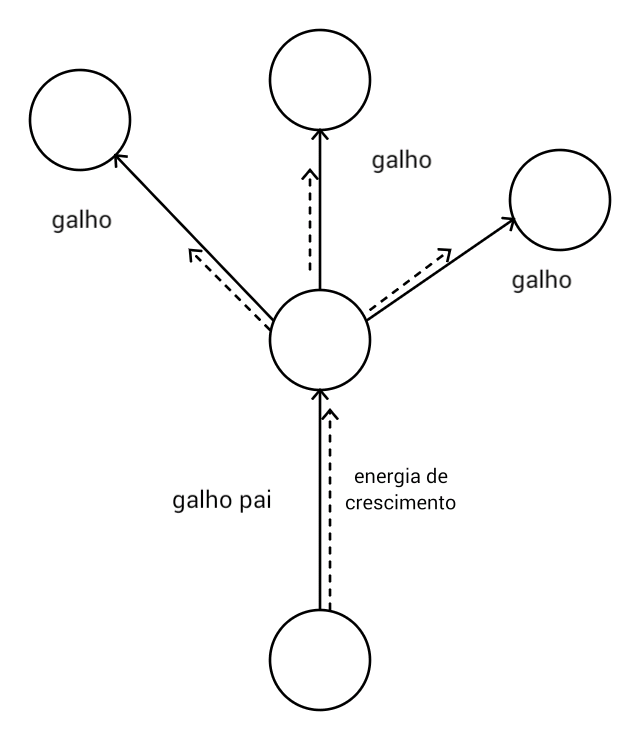
\includegraphics[scale=0.2]{img/PI3_Ponto_Crescimento.png}
		\caption{\footnotesize {Crescimento dos galhos e energia transferida de pai para filho.} }
	\end{center}
	\end{figure}	
	
\subsubsection{Crescimento}
Para que os galhos crescam controladamente mas mantendo certa diferencia\c c\~ao em tamanho e
dire\c c\~ao entre um e outro, estabelecemos um crit\'erio que chamamos de energia de crescimento e energia limite.
A energia limite determina o quanto cada  galho da \'arvore vai crescer e \'e estabelecido atrav\'es de uma porcentagem,
calculada a partir do total de energia de crescimento fornecida para o galho, o n\'ivel de altura desse galho e a energia
limite da \'arvore:

  \texttt{\footnotesize{galho.energiaLimite = (energiaRecebida * (arvore.energiaLimite - (galho.profundidade * 2)) / 100)}}

O valor da energia limite pode
ser alterado de acordo com a intera\c c\~ao do usu\'ario ao longo do jogo, o que pode proporcionar uma \'arvore mais
mais ou menos desenvolvida.

Enquanto os galhos crescem eles podem dar origem a novos galhos. Isso \'e determinado ap\'os ser consumida uma determinada
quantidade de energia de crescimento fornecida ao galho, o que permite que a simula\c c\~ao de crescimento da \'arvore
fique mais natural. A \'unica exce\c c\~ao \'e o tronco da \'arvore, que tem o crescimento
mais controlado:

\texttt{\footnotesize{\textbf{SE} galho.energiaConsumida < galho.energiaLimite \textbf{E} galho.energiaRecebida > 0
\textbf{ENT\~AO} galho.crescer}}

\subsubsection{Pontos de crescimento de frutos e folhas}
Os pontos de crescimento de frutos e folhas s\~ao determinados de acordo com o m\'inimo de energia que o galho
tem para crescer. Caso esse valor seja igual ou abaixo de determinado crit\'erio, o algoritmo de simula\c c\~ao assume
que n\~ao ir\~ao surgir novos galhos a partir do galho atual, ainda durante a fase de crescimento. Com isso determinado,
o galho passa a produzir folhas e frutos ao inv\'es de novas ramifica\c c\~ao de galhos.

	\begin{figure}[ht!]
	\begin{center}
		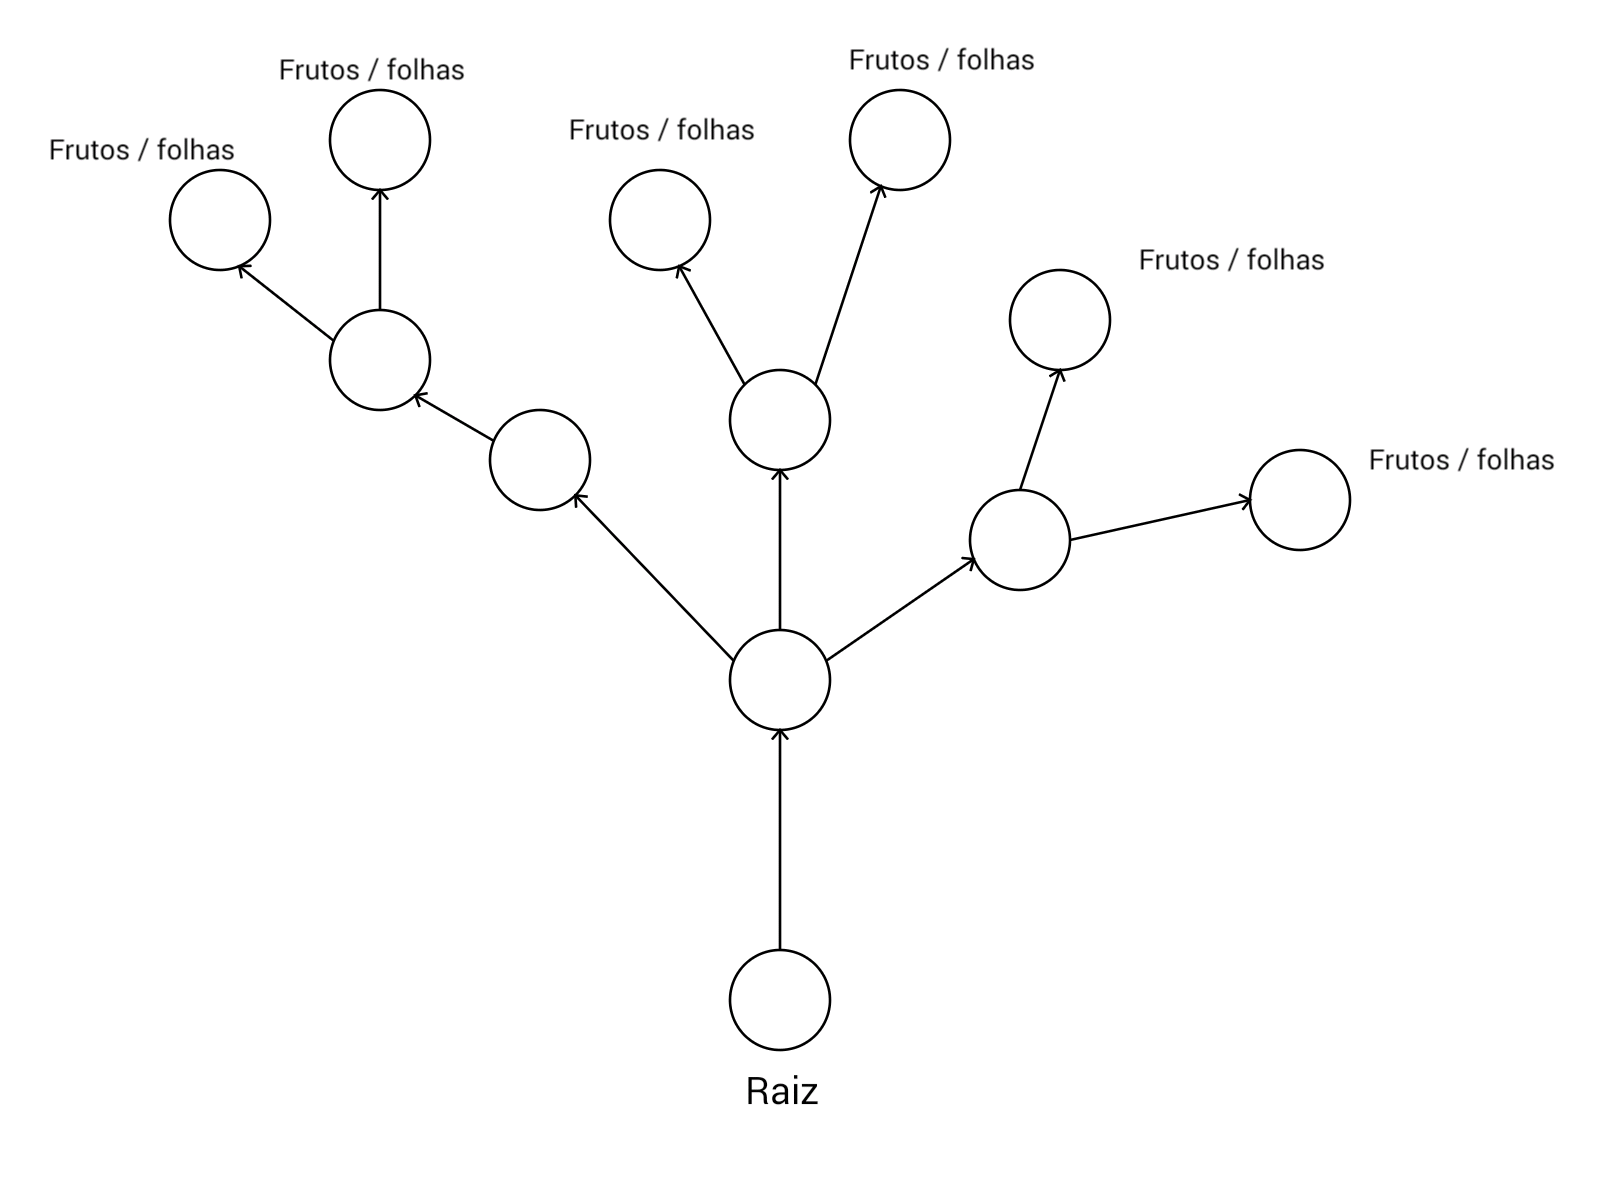
\includegraphics[scale=0.15]{img/PI3_Arvore.png}
		\caption{\footnotesize {Estrutura da \'arvore e pontos de crescimento de frutos e folhas.} }
	\end{center}
	\end{figure}	

\subsection{Primeiros experimentos}
Para o reconhecimento de uma cor emitida por um LED do Arduino, fizemos uma otimiza\c c\~ao f\'isica
com um peda\c co de papel que reduzisse o brilho da luz, por\'em ainda n\~ao \'e suficiente para
o reconhecimento total.

Como experimentos necess\'arios, temos o reconhecimento da luminosidade para verificar
a proximidade da luz com a c\^amera e uma otimiza\c c\~ao afim de isolar a cor do LED,
ignorando as outras cores similares e aparentes na c\^amera.

\section{Bibliotecas}
\subsection{OpenCV}
\subsection{Allegro}
\subsection{Arduino-Serial}

\section{Equipamentos}
\begin{itemize}
\item C\^amera de captura de v\'ideo
\item Placa controladora ARduino Uno
\item LED RGB
\item Computador (desktop ou notebook)
\end{itemize}

\nocite{*}

\section{Bibliografia}
\bibliographystyle{sbc}
\bibliography{plantgoshi}


\end{document}
